\documentclass[fontsize=11pt]{article}
\usepackage{amsmath}
\usepackage[utf8]{inputenc}
\usepackage[margin=0.75in]{geometry}
\usepackage{graphicx}
\usepackage{tabularx}

\title{CSC111 Final Project Report: Rhythm Radar - Underground Song Recommendation System}
\author{Olindi Mallika Appuhamilage, Mahek Cheema, Bea Alyssandra Castro, Kelsang Tsomo}
\date{Monday, April 03, 2023}

\begin{document}
\maketitle

\begin{enumerate}
\item \textbf{Problem Description and Project Question/Goal}
    \begin{enumerate}
    \item \textbf{Background} \newline
    Spotify is the world’s most popular audio streaming platform with over 11 million artists and creators and almost 500 million users. With over 100 million tracks from various genres on the platform, the app allows users to not only listen to their favourite music, but also allows users to create and save playlists based on their preferences. In order to suggest new tracks to users, Spotify’s current recommendation integrates collaborative filtering with content-based filtering. To create user-tailored recommendations, collaborative filtering examines a user's listening history. On the other hand, content-based filtering suggests music based on the features of a track, akin to mood, genre and danceability (Marius, 2021).  \newline

    \item\textbf{Problem Context and Motivation} \newline
    Due to the platform’s large catalogue of songs, it can make users feel overwhelmed and increase the difficulty of discovering new music and artists. Regardless of Spotify’s endeavours to curate personalized music recommendations, it can nevertheless be difficult for Spotify users to find new music, specifically from underground musicians. The primary reason for this is due to the platform’s recommendation algorithm being built to give preference to popular mainstream music and artists to attract a wider audience. For instance, many of Spotify’s playlist recommendations are created by the platform’s team or influential users, which tend to give spotlight to well-established artists. The exposure and publicity of a track on Spotify is significantly influenced by these playlists in addition to the recommendation algorithm especially. Hence, underground and new artists are underrepresented on the platform, as it is difficult to get their music featured on these curated playlists, due to fewer resources and finances, which limits their possibilities of reaching new listeners (Mitchell, 2022). \newline
    
    \item \textbf{Goal} \newline
    To address this issue, we seek \textbf{to develop a music recommendation system that curates playlists from the users preferred playlist while simultaneously putting emphasis on underground songs to support small and emerging musicians.} The new algorithm will suggest a playlist of ten songs by lesser-known artists using a myriad of song features, such as energy, danceability, valence, loudness and popularity from the user's current playlist, compared to the songs in the spotify database. From the user’s playlist, we will randomly select ten songs to perform computations on, and in return a total of ten new songs based on these ten songs will be returned to the user. \newline
    \end{enumerate}

\item\textbf{Datasets}
    \begin{enumerate}
    \item data.csv \newline
    This Spotify data file contains up to 1.2 million songs, with columns named ‘year’, ‘id’, ‘artists’, ‘popularity’, ‘danceability’, ‘instrumental’, ‘name’, ‘release date’, ‘valence’ and more. Some sample data in this dataset with the relevant data for our program is shown below:
    \newline

    \begin{tabularx}{1\textwidth} { 
    | >{\centering\arraybackslash}X 
    | >{\centering\arraybackslash}X 
    | >{\centering\arraybackslash}X 
    | >{\centering\arraybackslash}X 
    | >{\centering\arraybackslash}X 
    | >{\centering\arraybackslash}X 
    | >{\centering\arraybackslash}X 
    | >{\centering\arraybackslash}X 
    | >{\centering\arraybackslash}X }

    \hline
    
    id & artist & name & valence & energy & popularity & danceability & loudness\\
    \hline
    7xPhfUa
    n2yNtyFG
    0cUWkt8  & ‘Dennis Day’ & ‘Clancy Lowered the Boom’ & 0.963 & 0.341 & 5 & 0.819 & -12.441\\
    \hline
    \end{tabularx} \newline
    
This data is accessible on Kaggle Datasets, https://www.kaggle.com/code/vatsalmavani/music-recommendation-system-using-spotify-dataset/input \newline

    \end{enumerate}

\item\textbf{Computational Overview}
    \begin{enumerate}
    \item\textbf{visualization.py} \newline
        Our user interface for our song recommendation system was created by incorporating the use of two Python libraries: Tkinter and Pyperclip. The main windows were created using Tkinter and contains a title label, a subtitle label, an instructions label, an input box for the user to enter their Spotify playlist link, a "Go" button to submit the link, and a "Paste" button to paste the link from the user's clipboard. Pyperclip was used to access the user's clipboard and retrieve any text that had been copied to it, as it is a library that provides a cross-platform interface for working with the clipboard in Python.Specifically, the on\_paste() function was called when the user clicked the "Paste" button, and this function used the pyperclip.paste() method to retrieve the text from the clipboard. Once the text was retrieved, the input\_box Entry widget was updated to display the pasted text using the insert() method. This allowed the user to quickly and easily input a Spotify link without having to manually type it out. By using pyperclip, the code is able to provide a more user-friendly interface for entering a Spotify link, and makes it easier for users to use the application. The user should be able to interact with the two windows created: the first being where the user should input their playlist, and the second window will show a list of ten new songs from their playlist, that the user can then either like or dislike. \\
        \begin{enumerate}
            \item {The ‘SongRecommendation’ class:}
            \begin{enumerate}
                \item This class takes a Spotify link as input when initialized and has a method get\_recommendations that returns a list of recommended songs based on the input link. \\
            \end{enumerate}
            
            \item {The ‘RecommendationWindow’ class:}
            \begin{enumerate}
                \item This class created a new window using Tkinter to display the recommended songs to the user. It takes a list of recommended songs as its input and creates a frame for each song in the list, where each frame contains a label displaying the name of the song and two checkbuttons, one for “like” and one for “dislike,” where the user can click to rate the song.

                \item We also created a method called ‘update\_song\_rate’ which updates a dictionary called ‘song\_ratings’ that stores the user’s ratings for each song. \\
            \end{enumerate}

            \item {The ‘LinkHolder’ class:}
            \begin{enumerate}
                \item This was extremely important to our interface, as we needed a class to store the user’s inputted public Spotify playlist link in order to extract its data and perform computations on the given songs. \\
            \end{enumerate}

            \item {The $‘$on\_submit$’$ function:}
            \begin{enumerate}
                \item This function is only called when the user either clicks enter on their keyboard or the “Go” button in the main window. It gets the link from the input box, creates a SongRecommendation object with the link, calls the get\_recommendations method to generate a list of recommended songs, and then creates a RecommendationWindow object to display the recommendations to the user. It also clears the input box after the user clicks "Go". \\
            \end{enumerate}
            
            \item {The $‘$on\_paste$’$ function:}
            \begin{enumerate}
                \item This function is only called when the user clicks the “Paste” button in the main window, where it inserts the text from the user’s clipboard into the input box. \\
            \end{enumerate}
        \end{enumerate}
        
        In addition to these classes and functions, we also used a variety of Tkinter’s functions, such as a significant one being ‘Entry,’ which creates an entry widget that allows the user to enter their public spotify link. We also used ‘Button,’ which creates a button widget that can be clicked to perform an action, which was specifically used to create the “Go” and “Paste” buttons. Furthermore, the ‘mainloop()’ function starts the main event loop, which listens for events such as button clicks, key presses, and mouse movements. It runs continuously until the user closes the window or the program is terminated. In the code, we use this function to start the event loop for the main window and for the song recommendation window. \\

        \item\textbf{playlist.py}
        \begin{itemize}\item Song class in playlist.py
        \end{itemize}
        Song class in playlist.py is analogous to the \_Vertex class we are familiar with, where every vertex in the graph represents a song in the user’s playlist. We create the Song class with public instance attributes consisting of song\_id(str), name(str), artists(str), valence(float), danceability(float), and others.

        \begin{itemize}\item Channel class in playlist.py
        \end{itemize}
        Channel class represents a link between two songs in an interconnection network and includes a function called get\_other\_endpoint that collects thats linked by its channel.

        \begin{itemize}\item Playlist class in playlist.py
        \end{itemize}
        Playlist class is a graph, or more specifically, an AbstractNetwork, which collects songs in our database. Every vertex/song in the graph is one song and collects ten random songs from the users playlist that are each connected to their similar songs. The Playlist class includes a private instance attribute called \_songs, which is a dictionary that maps the song’s unique ID to its Song object. 
        \newline

        First, both the user’s playlist and our dataset must get filtered. The first filtering function is  get\_playlist\_songs, which takes a random sample of 20 random song ids from the user’s input playlist. The second filtering function, get\_dataset\_songs, loads all songs in the dataset csv file and adds a new Song object containing the song id, the artist name, the title of the song, danceability, valence, energy, and loudness respectively.
        \newline

        In order to find similar songs to recommend to the user, the computation function getsongs\_in\_range is used. A “similar song” is found by sorting through each song from the dataset and keeping the songs that are within a certain range of each Song attribute of ten random songs from the user’s playlist. In our case, a “similar song” must have a danceability within a range of -0.2 and 0.2, a valence within a range of -0.2  0.2, have an energy within a range of -0.5 and +0.5, have a loudness within a range of -2 and +2. We found that these values for the ranges gave the user the best results. If these requirements are met, a new channel is added from each of the randomly selected user’s playlist songs and the “similar song” from the dataset.
    

        \item\textbf{score\_computations.py}
        \begin{itemize}\item Computations class in score\_computations.py
        \end{itemize}
        
        \begin{itemize}
         \item Computations class is responsible for computing the distance of the user’s current song and the current data csv song.
         \newline
         \newline
         \item Another filtering occurs in remove\_out\_of\_range, where the songs that do not have channels, meaning the songs that there were either no songs from the dataset that were within the user's songs' danceability, valence, energy, and loudness or the similar song found from the dataset is the same song from the user's playlist, are removed.
         

         \item To find the distance between the user’s song and the current song from our spotify dataset, the computation function euclidean\_distance is used. In this function, we iterate through all active channels and access the valence, danceability, energy, and loudness again then perform distance = \sqrt{[(x2 – x1)^2 + (y2 – y1)^2]}.
        \end{itemize}
        Our program uses a new library called Spotipy allows us to readily access the Spotify Web API where we can obtain information about artists, albums, playlists and tracks. This Python library will be used to gather necessary data about the songs found in the user's playlist and songs in Spotify’s database that will be recommended to users, specifically the song characteristics akin to key, danceability, popularity, valence, tempo and more. Spotipy features the following function, sp.audio\_features(tracks=[]), which returns the audio features for a list of songs. The public playlist inputted from the user can provide us with a catalogue of track IDs that we can pass into the function. \\
        
    \end{enumerate}

\textbf{4. Obtaining Datasets and Running the Program} \newline

    \begin{enumerate}

        \item [1] Download new\_small.csv
        \item [2] Run main.py in python console
        \item [3] After RhythmRadar appears on the screen, copy and paste a Spotify Playlist that has over 10 songs into the textbox and press the “Go” button.
        \item[4] *Because of the error we are experiencing, we were not able to display the suggest playlist because we cant access the methods used to display and compute the similar songs. We believe the because of this is something to do with the command queue or our input function.*
    \end{enumerate}
    
\item \textbf{Visualization/Interactive Model} 

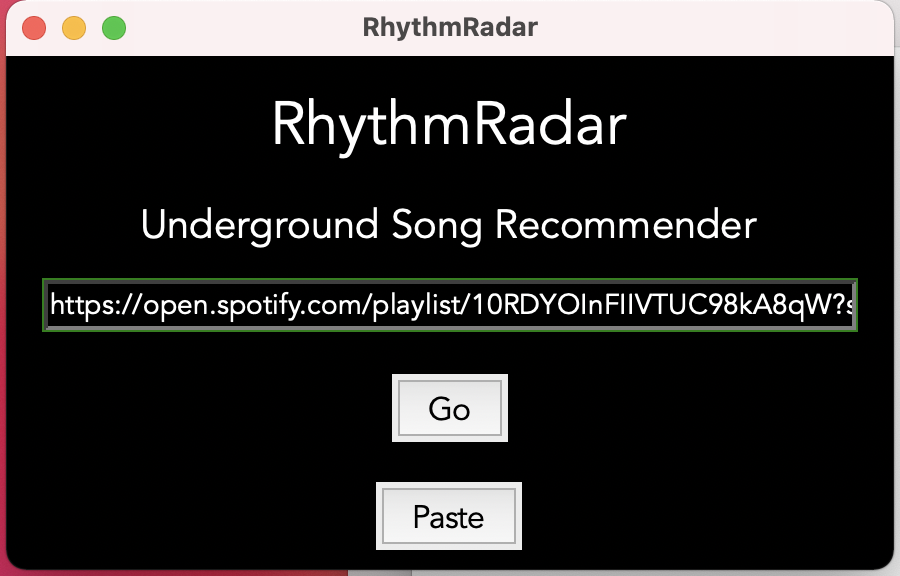
\includegraphics[width=.8\textwidth]{rr_main.png} \newline
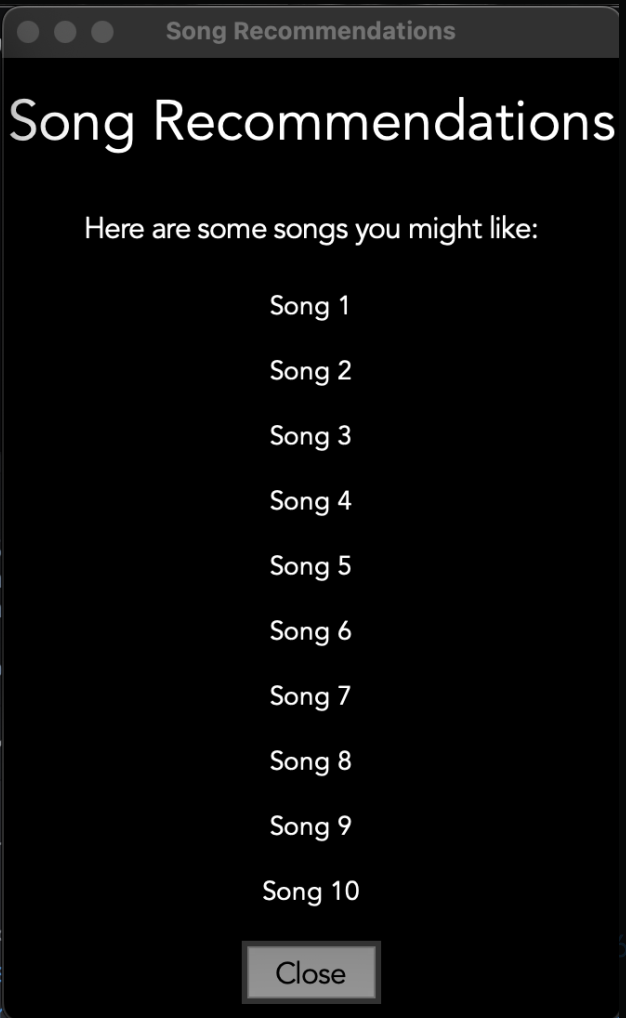
\includegraphics[width=.5\textwidth]{recommendation.png}

         Another filtering occurs in remove\_out\_of\_range, where the songs that do not have channels, meaning the songs that there were either no songs from the dataset that were within the user's songs' danceability, valence, energy, and loudness or the similar song found from the dataset is the same song from the user's playlist, are removed.
         \newline
         To find the distance between the user’s song and the current song from our spotify dataset, the computation function euclidean\_distance is used. In this function, we iterate through all active channels and access the valence, danceability, energy, and loudness again then preform $distance$ = \sqrt{[(x2 – x1)^2 + (y2 – y1)^2]}.
    *Because of the error we are experiencing, we were not able to display the suggest playlist because we cant access the methods used to display and compute the similar songs. We believe the because of this is something to do with the command queue or our input function.*
\item\textbf{Changes from Initial Proposal}
During the course of completing this project, we made a myriad of changes from the initial plan outlined in the project proposal. One of the most significant changes was found in ‘visualization.py,’ where we switched the method of which we would create a user interface and visualize our results. Our initial plan was to use the Python library, Pygame, such as using pygame.Surface to create various shapes, akin to boxes and circles and create text. We also wanted to manage human interactions through mouse clicks and keyboard strokes by using Pygame’s event module. However, the main issue lied in not only creating an interactive text input box for the user to input their public spotify playlist link, but also ensuring that we stored this link in order to extract the data from this link and ultimately perform computations. It was thus harder for Pygame to support user-inputted data such as the playlist link. In addition, it was also difficult to ensure that users can copy-paste their links, which at its previous state, users needed to manually input their code which is inefficient and not user friendly. We wanted to prioritize the user-friendliness of our program and thus came to the conclusion that it would be best to change the approach of our visualization. As a result of this, we eventually decided to use the library, Tkinter, instead to better serve our purposes. Switching to Tkinter allowed us to create a more user-friendly interface and integrate our recommendation engine more seamlessly into the application. We were able to create a clean and intuitive interface with Tkinter, which made it easier for users to input their Spotify link and view their recommended songs. While it took some time to learn how to use Tkinter effectively, we ultimately found it to be a valuable addition to our project. Regarding the feedback section, it was more difficult to implement in Pygame because we had to manually store and manage the user's feedback, as well as display it in a user-friendly way. With Tkinter, we were able to use built-in widgets such as Checkbuttons to easily capture the user's feedback and display it in real-time. This made it easier for users to provide feedback on the recommended songs, and for us to store and analyze that feedback. \newline

In addition to swapping the Python library Pygame to Tkinter, we further decided to use another Python library called Pyperclip. In our project, we needed to allow users to paste their Spotify link into our program. However, we quickly realized that the standard Tkinter entry widget did not support pasting, which made it less user-friendly. To solve this problem, we decided to use a new Python library called "pyperclip". Pyperclip is a cross-platform module that allows us to copy and paste text to and from the clipboard. With Pyperclip, we were able to easily implement a "Paste" button that would allow users to paste their Spotify link into our program. Overall, using Pyperclip was a great solution to our problem and made our program more user-friendly. Pyperclip was easier to combine with Tkinter in comparison to Pygame, and thus we thought this change from our initial proposal was successful and enhanced our program. \newline

The dataset we decided to use contained 19 different columns, where we initially decided to use all of the columns to compute a list of similar songs, such as ‘instrumentalness,’ and ‘liveness.’ However, when we began to put together a plan on calculating the similarity between songs, we realized that using all of these features would not be helpful to our program, as some of these columns were not comparable with each other. For instance, it is difficult to compare the key of a song to its liveness or instrumentalness. Thus, we needed to calculate the distance between similar variables. To accomplish this, we decided to only use the variables that would be relevant to the program and can be compared using the Euclidean distance formula in order to accurately return similar songs. We decided to thus only use ‘id,’ ‘artist,’ ‘popularity,’ ‘danceability,’ ‘loudness,’ ‘energy,’ ‘valence’ and ‘name,’ from the file. We were then able to compare the loudness and energy of the songs, which are similar variables that can be compared using the Euclidean distance. Similarly, we compared the valence and danceability of the songs, as they are also similar variables. By doing this, we were able to calculate the Euclidean distance between songs and determine their similarity, which would have been otherwise hindered if we did not select the most relevant columns to use from the dataset. Euclidean distance is a mathematical formula that calculates the distance between two points in space. In our case, the points are the different audio features of a song. By calculating the Euclidean distance between two songs, we were able to determine their similarity. The smaller the distance, the more similar the songs were. This approach allowed us to create a more accurate and effective song recommender. \newline

The use of the graph abstract data type was another change we made. Initially, we planned to have two classes called Song and Playlist, where Song would represent a single song and Playlist would represent the ten songs selected from the user's playlist. However, we realized that we needed another class to represent the connections between the songs. Although we did have an attribute called ‘recommended\_songs,’ which represented songs similar to the given song, we wanted to further represent a connection between songs in order to perform computations effectively. As a result, we created another class called Channel, which connected two songs in our playlist. We were then able to use these channels in our ‘remove\_out\_of\_range’ and ‘similar\_songs\_helper.’ A song without channels means there were either no songs from the dataset that were within the user’s songs’ danceability, loudness, energy and valence or the similar song found from the dataset is the same song from the user’s playlist. This allowed us to organize our data in a more effective way. 

\item\textbf{Discussion}
\begin{enumerate}
    \item\textbf{Interpretation and Analysis of Results} \newline
    The goal of our project was to develop a music recommendation system that curates playlists from the users preferred playlist while simultaneously putting emphasis on underground songs to support small and emerging musicians. While the results of our project do achieve this goal, as the user is given ten new songs from small and emerging musicians, the extent to which this goal was reached is subject to the user themselves. Determining how similar two songs are is extremely subjective and intricate, which was the biggest challenge throughout the duration of completing this assignment. Music involves various elements, such as melody, rhythm and instrumentation, hence, there is no definitive way of judging the similarity of songs objectively, regardless of using numerical data on the measures of loudness and energy etc. Although these elements were quantified and used to determine the similarity between songs, there still may be minor errors or discrepancies that can affect the overall similarity measurement. For example, two songs may have a similar degree of danceability and energy, but one song may have a more complex melody or a more catchy and memorable chorus. As a result, our program's recommendation may not always align with the user's subjective taste, as they may prefer a song with a simpler melody or a different tone. Our program does not allow the user to choose which aspects of the songs they want to be similar, such as lyrics, instrumentation, or tempo, which further limits the accuracy of the recommendations. However, we tried to minimize this limitation by providing users with a feedback system where they can indicate whether they liked or disliked a song. This feedback system allows the program to learn more about the user's preferences and improve the recommendations it provides over time. Therefore, it is important to acknowledge the subjectivity involved in determining song similarity and to set specific criteria for evaluating the success of a recommendation system, such as the likeability of the recommended songs by the user. Due to this subjectivity, we collectively believe that our program is successful if it recommends songs by artists that the user has not heard of previously, and if they ‘like’ the song, which is open to interpretation by the user. \newline

    The program effectively suggested new songs that we had never heard before when we tried it using our own playlists and the playlists of our friends. This was especially thrilling because finding new, obscure music was one of our program's main objectives. The suggestions were given in a way that was both clear and simple to comprehend, which improved the user experience all around. We computed the similarity between the songs based on the Euclidean distance, which was useful in calculating the distance between a song from our dataset and a song selected by the user. However, the Euclidean distance had limitations, as it did not allow us to compare a more comprehensive range of variables, such as key, mode, tempo, and instrumentalness, which could have affected our output's accuracy. While the variables we used, such as energy, danceability, loudness, and valence, provided us with a decent representation of the songs' similarity, they were not an exhaustive list of characteristics that contribute to the overall similarity of two songs. Therefore, we acknowledge that our program's output may not have been entirely precise and may have missed some similarities or differences between the songs. Nonetheless, we believe that it still provided useful recommendations to the user, as evidenced by the positive feedback we received.\newline
    
    Even though we had trouble visualizing the outcomes, we still think that the program was made with user-friendliness in mind, as users found it simple to comprehend and navigate through the program's findings, which were presented in an organized and straightforward manner. In order to further customize the suggestions, our program also gave users the option to like or dislike the tracks that were suggested. \newline

    \item\textbf{Limitations} \newline
    One limitation we encountered was related to the datasets we used. While we were able to access a vast amount of song data through the Spotify API, we found that our dataset did not include every song in Spotify's database. This meant that some less popular songs may not be included in our recommendations, which could limit the diversity of our recommendations. Additionally, we were only able to access information on a limited number of variables that comprise a song, which may have further impacted the accuracy of our recommendations. \newline

    The algorithms and tools we used in our project were another limitation we ran into. As an example, I already stated that one of the biggest difficulties we encountered was creating an interactive interface that could work in unison with our suggestion engine. Initially, we tried using Pygame to enable user-inputted data like the playlist link, but we soon realized that it was not the best solution for this because we had trouble making sure that users could copy and paste their links, which made entering the playlist code more difficult. We ultimately changed to the Tkinter library to overcome this restriction, which enabled us to develop a more streamlined user interface that was easily combined with our recommendation engine. \newline

    Furthermore, because the user might prefer music with a simplified rhythm or in a particular language, our program's suggestion might not always match their individual preferences. Any music recommendation system has this limitation by nature because it is challenging to anticipate each person's tastes with full precision. Additionally, our program does not let users specify which musical characteristics, such as lyrics, instrumentation, or tempo, they want the songs to be comparable to, which may reduce the precision of the suggestions and make the program less user-friendly. Nevertheless, we believe that our program provides a useful starting point for users looking to discover new music based on their inputted playlist. \newline

    \item\textbf{Next Steps} \newline
    There are several potential next steps for further exploration in this project: \\
    \begin{enumerate}
        \item \emph{Incorporate more variables:} Currently, our program only takes into account a few variables such as energy, danceability, loudness, and valence. Adding more variables such as lyrics, tempo, key, and mode could potentially improve the accuracy of our recommendations.\\
        
        \item \emph{Improve user interface:} While our user interface is user-friendly, there is still room for improvement, for example, we could add more visualizations to help users better understand the recommendations or add more customization options so users can toggle which aspects of the songs they want to be similar. We can also allow users to select which specific genres they would like the music to reflect. The interface currently only supports public spotify playlist links; however, to further enhance this, we can allow users to simply search for one song and find a multitude of songs that are similar to their input. The same can be done for albums as well, giving the user more variety. \\
        
        \item \emph{Implement machine learning algorithms:} We could explore using machine learning algorithms such as K-Nearest Neighbors to improve our recommendation engine, as our current implementation utilized the Euclidean distance instead. These algorithms could potentially improve the accuracy of our recommendations by taking into account more data and learning from past user behavior.\\
    \end{enumerate}


     
    \end{enumerate}
\end{enumerate}

\section{References}
Mitchell, Tay. “Spotify’s Algorithm: Helping or Hurting Musicians?” Arts Management \& Technology Laboratory, 28, Apr. 2022, https://amt-lab.org/blog/2022/4/spotifys-algorithm-helping-or-hurting. Accessed 7 Mar. 2023.\\ 

Marius, Hucker. “Uncovering How the Spotify Algorithm Works.” Towards Data Science, 23 Nov. 2021, https://towardsdatascience.com/uncovering-how-the-spotify-algorithm-works-4d3c021ebc0. Accessed 7 Mar. 2023 \\

“Web API.”  Spotify for Developers. https://developer.spotify.com/documentation/web-api/. Accessed 6 Mar. 2023. \\

Lamere, Paul. “Welcome to Spotipy!” spotipy, 2014, https://spotipy.readthedocs.io/en/2.22.1/. Accessed 6 Mar. 2023. \\

Watts, Cameron. “Extracting Song Data From the Spotify API Using Python.” Towards Data Science, 17 Dec. 2021, https://towardsdatascience.com/extracting-song-data-from-the-spotify-api-using-python-b1e79388d50. Accessed 7 Mar. 2023. \\

Ashrith. “What Makes a Song Likeable? - towards Data Science.” Medium, Towards Data Science, 4 Dec. 2018, towardsdatascience.com/what-makes-a-song-likeable-dbfdb7abe404. Accessed 7 Mar. 2023. \\

Ankthon. “Python | random.sample() function.” GeeksforGeeks, 29 Aug. 2018, https://www.geeksforgeeks.org/python-random-sample-function/.  \\

Al-Masri, Anas. “How does k-Means Clustering in Machine Learning Work?” TowardsDataScience, 14, May 2019. https://towardsdatascience.com/how-does-k-means-clustering-in-machine-learning-work-fdaaaf5acfa0. \\

Schafer, Corey. “Matplotlib Tutorial (Part 7): Scatter Plots.” Youtube, uploaded by Corey Schafer, 16 Jun. 2019, https://www.youtube.com/watch?v=zZZ\_RCwp49g \\


\end{document}
